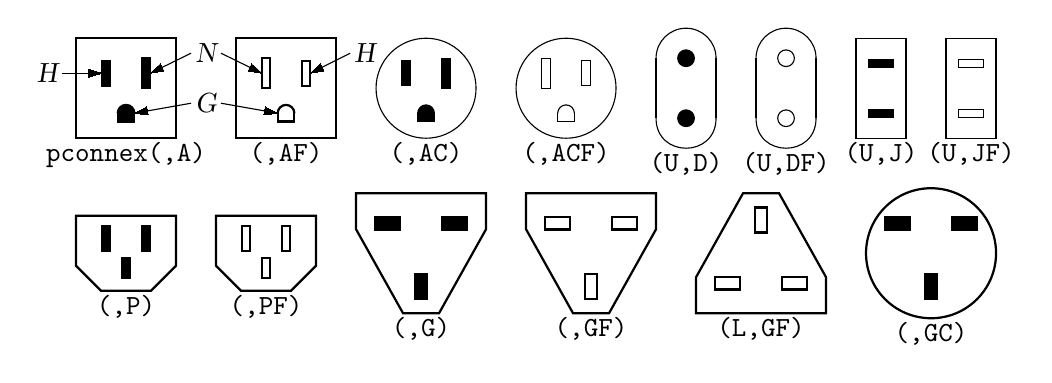
\begin{tikzpicture}[scale=2.54]
% dpic version 2020.03.01 option -g for TikZ and PGF 1.01
\ifx\dpiclw\undefined\newdimen\dpiclw\fi
\global\def\dpicdraw{\draw[line width=\dpiclw]}
\global\def\dpicstop{;}
\dpiclw=0.8bp
\dpiclw=0.8bp
\dpicdraw (0.598611,0.013889)
 --(0.598611,0.263889)
 --(0.098611,0.263889)
 --(0.098611,-0.236111)
 --(0.598611,-0.236111)
 --(0.598611,0.013889)\dpicstop
\global\let\dpicshdraw=\dpicdraw\global\def\dpicdraw{}
\global\def\dpicstop{--}
\dpicshdraw[fill=white!0!black]
\dpicdraw (0.469444,0.088889)
 --(0.469444,0.163889)
 --(0.427778,0.163889)
 --(0.427778,0.013889)
 --(0.469444,0.013889)
 --(0.469444,0.088889)\dpicstop
cycle; \global\let\dpicdraw=\dpicshdraw\global\def\dpicstop{;}
\global\let\dpicshdraw=\dpicdraw\global\def\dpicdraw{}
\global\def\dpicstop{--}
\dpicshdraw[fill=white!0!black]
\dpicdraw (0.269444,0.088889)
 --(0.269444,0.151389)
 --(0.227778,0.151389)
 --(0.227778,0.026389)
 --(0.269444,0.026389)
 --(0.269444,0.088889)\dpicstop
cycle; \global\let\dpicdraw=\dpicshdraw\global\def\dpicstop{;}
\fill[fill=black,line width=0bp](0.390278,-0.111111)
 ..controls (0.390278,-0.088099) and (0.371623,-0.069444)
 ..(0.348611,-0.069444)
 ..controls (0.325599,-0.069444) and (0.306944,-0.088099)
 ..(0.306944,-0.111111)--cycle
\dpicstop
\dpicdraw (0.390278,-0.111111)
 ..controls (0.390278,-0.088099) and (0.371623,-0.069444)
 ..(0.348611,-0.069444)
 ..controls (0.325599,-0.069444) and (0.306944,-0.088099)
 ..(0.306944,-0.111111)\dpicstop
\fill[fill=black,line width=0bp](0.306944,-0.111111)
 --(0.306944,-0.152778)
 --(0.390278,-0.152778)
 --(0.390278,-0.111111)--cycle
\dpicstop
\dpicdraw (0.306944,-0.111111)
 --(0.306944,-0.152778)
 --(0.390278,-0.152778)
 --(0.390278,-0.111111)\dpicstop
\dpiclw=0.4bp
\filldraw[line width=0bp](0.161111,0.068889)
 --(0.227778,0.088889)
 --(0.161111,0.108889) --cycle\dpicstop
\dpicdraw (0.218111,0.088889)
 --(0.027778,0.088889)\dpicstop
\draw (0.027778,0.088889) node[left=-2bp]{\sl H};
\dpiclw=0.8bp
\draw (0.348611,-0.236111) node[below=-2bp]{\tt pconnex(,A)};
\dpicdraw (1.398611,0.013889)
 --(1.398611,0.263889)
 --(0.898611,0.263889)
 --(0.898611,-0.236111)
 --(1.398611,-0.236111)
 --(1.398611,0.013889)\dpicstop
\dpicdraw (1.069444,0.088889)
 --(1.069444,0.163889)
 --(1.027778,0.163889)
 --(1.027778,0.013889)
 --(1.069444,0.013889)
 --(1.069444,0.088889)\dpicstop
\dpicdraw (1.269444,0.088889)
 --(1.269444,0.151389)
 --(1.227778,0.151389)
 --(1.227778,0.026389)
 --(1.269444,0.026389)
 --(1.269444,0.088889)\dpicstop
\dpicdraw (1.190278,-0.111111)
 ..controls (1.190278,-0.088099) and (1.171623,-0.069444)
 ..(1.148611,-0.069444)
 ..controls (1.125599,-0.069444) and (1.106944,-0.088099)
 ..(1.106944,-0.111111)\dpicstop
\dpicdraw (1.106944,-0.111111)
 --(1.106944,-0.152778)
 --(1.190278,-0.152778)
 --(1.190278,-0.111111)\dpicstop
\dpiclw=0.4bp
\filldraw[line width=0bp](1.320129,0.136592)
 --(1.269444,0.088889)
 --(1.338017,0.100815) --cycle\dpicstop
\dpicdraw (1.278091,0.093212)
 --(1.469444,0.188889)\dpicstop
\draw (1.469444,0.188889) node[right=-2bp]{\sl H};
\draw (0.748611,0.188889) node{\sl N};
\filldraw[line width=0bp](0.520518,0.136175)
 --(0.469444,0.088889)
 --(0.538113,0.100252) --cycle\dpicstop
\dpicdraw (0.673611,0.188889)
 --(0.478126,0.093141)\dpicstop
\filldraw[line width=0bp](0.95911,0.100252)
 --(1.027778,0.088889)
 --(0.976704,0.136175) --cycle\dpicstop
\dpicdraw (0.823611,0.188889)
 --(1.019096,0.093141)\dpicstop
\draw (0.748611,-0.061111) node{\sl G};
\filldraw[line width=0bp](0.452454,-0.07983)
 --(0.390278,-0.111111)
 --(0.459406,-0.119221) --cycle\dpicstop
\dpicdraw (0.673611,-0.061111)
 --(0.399798,-0.109431)\dpicstop
\filldraw[line width=0bp](1.037817,-0.119221)
 --(1.106944,-0.111111)
 --(1.044768,-0.07983) --cycle\dpicstop
\dpicdraw (0.823611,-0.061111)
 --(1.097425,-0.109431)\dpicstop
\draw (1.148611,-0.236111) node[below=-2bp]{\tt (,AF)};
\dpicdraw (1.848611,0.013889) circle (0.098425in)\dpicstop
\global\let\dpicshdraw=\dpicdraw\global\def\dpicdraw{}
\global\def\dpicstop{--}
\dpicshdraw[fill=white!0!black]
\dpicdraw (1.969444,0.088889)
 --(1.969444,0.163889)
 --(1.927778,0.163889)
 --(1.927778,0.013889)
 --(1.969444,0.013889)
 --(1.969444,0.088889)\dpicstop
cycle; \global\let\dpicdraw=\dpicshdraw\global\def\dpicstop{;}
\global\let\dpicshdraw=\dpicdraw\global\def\dpicdraw{}
\global\def\dpicstop{--}
\dpicshdraw[fill=white!0!black]
\dpicdraw (1.769444,0.088889)
 --(1.769444,0.151389)
 --(1.727778,0.151389)
 --(1.727778,0.026389)
 --(1.769444,0.026389)
 --(1.769444,0.088889)\dpicstop
cycle; \global\let\dpicdraw=\dpicshdraw\global\def\dpicstop{;}
\fill[fill=black,line width=0bp](1.890278,-0.111111)
 ..controls (1.890278,-0.088099) and (1.871623,-0.069444)
 ..(1.848611,-0.069444)
 ..controls (1.825599,-0.069444) and (1.806944,-0.088099)
 ..(1.806944,-0.111111)--cycle
\dpicstop
\dpicdraw (1.890278,-0.111111)
 ..controls (1.890278,-0.088099) and (1.871623,-0.069444)
 ..(1.848611,-0.069444)
 ..controls (1.825599,-0.069444) and (1.806944,-0.088099)
 ..(1.806944,-0.111111)\dpicstop
\fill[fill=black,line width=0bp](1.806944,-0.111111)
 --(1.806944,-0.152778)
 --(1.890278,-0.152778)
 --(1.890278,-0.111111)--cycle
\dpicstop
\dpicdraw (1.806944,-0.111111)
 --(1.806944,-0.152778)
 --(1.890278,-0.152778)
 --(1.890278,-0.111111)\dpicstop
\draw (1.848611,-0.236111) node[below=-2bp]{\tt (,AC)};
\dpicdraw (2.548611,0.013889) circle (0.098425in)\dpicstop
\dpicdraw (2.469444,0.088889)
 --(2.469444,0.163889)
 --(2.427778,0.163889)
 --(2.427778,0.013889)
 --(2.469444,0.013889)
 --(2.469444,0.088889)\dpicstop
\dpicdraw (2.669444,0.088889)
 --(2.669444,0.151389)
 --(2.627778,0.151389)
 --(2.627778,0.026389)
 --(2.669444,0.026389)
 --(2.669444,0.088889)\dpicstop
\dpicdraw (2.590278,-0.111111)
 ..controls (2.590278,-0.088099) and (2.571623,-0.069444)
 ..(2.548611,-0.069444)
 ..controls (2.525599,-0.069444) and (2.506944,-0.088099)
 ..(2.506944,-0.111111)\dpicstop
\dpicdraw (2.506944,-0.111111)
 --(2.506944,-0.152778)
 --(2.590278,-0.152778)
 --(2.590278,-0.111111)\dpicstop
\draw (2.548611,-0.236111) node[below=-2bp]{\tt (,ACF)};
\dpicdraw (3.298611,-0.136111)
 --(3.298611,0.163889)\dpicstop
\dpicdraw (3.298611,0.163889)
 ..controls (3.298611,0.246732) and (3.231454,0.313889)
 ..(3.148611,0.313889)
 ..controls (3.065768,0.313889) and (2.998611,0.246732)
 ..(2.998611,0.163889)\dpicstop
\dpicdraw (2.998611,0.163889)
 --(2.998611,-0.136111)\dpicstop
\dpicdraw (2.998611,-0.136111)
 ..controls (2.998611,-0.336111) and (3.298611,-0.336111)
 ..(3.298611,-0.136111)\dpicstop
\global\let\dpicshdraw=\dpicdraw\global\def\dpicdraw{}
\global\def\dpicstop{--}
\dpicshdraw[fill=white!0!black]
\dpicdraw (3.148611,0.163889) circle (0.016404in)\dpicstop
cycle; \global\let\dpicdraw=\dpicshdraw\global\def\dpicstop{;}
\global\let\dpicshdraw=\dpicdraw\global\def\dpicdraw{}
\global\def\dpicstop{--}
\dpicshdraw[fill=white!0!black]
\dpicdraw (3.148611,-0.136111) circle (0.016404in)\dpicstop
cycle; \global\let\dpicdraw=\dpicshdraw\global\def\dpicstop{;}
\draw (3.148611,-0.286111) node[below=-2bp]{\tt (U,D)};
\dpicdraw (3.798611,-0.136111)
 --(3.798611,0.163889)\dpicstop
\dpicdraw (3.798611,0.163889)
 ..controls (3.798611,0.246732) and (3.731454,0.313889)
 ..(3.648611,0.313889)
 ..controls (3.565768,0.313889) and (3.498611,0.246732)
 ..(3.498611,0.163889)\dpicstop
\dpicdraw (3.498611,0.163889)
 --(3.498611,-0.136111)\dpicstop
\dpicdraw (3.498611,-0.136111)
 ..controls (3.498611,-0.336111) and (3.798611,-0.336111)
 ..(3.798611,-0.136111)\dpicstop
\dpicdraw (3.648611,0.163889) circle (0.016404in)\dpicstop
\dpicdraw (3.648611,-0.136111) circle (0.016404in)\dpicstop
\draw (3.648611,-0.286111) node[below=-2bp]{\tt (U,DF)};
\dpicdraw (4.248611,0.013889)
 --(4.248611,0.263889)
 --(3.998611,0.263889)
 --(3.998611,-0.236111)
 --(4.248611,-0.236111)
 --(4.248611,0.013889)\dpicstop
\global\let\dpicshdraw=\dpicdraw\global\def\dpicdraw{}
\global\def\dpicstop{--}
\dpicshdraw[fill=white!0!black]
\dpicdraw (4.123611,0.159722)
 --(4.061111,0.159722)
 --(4.061111,0.118056)
 --(4.186111,0.118056)
 --(4.186111,0.159722)
 --(4.123611,0.159722)\dpicstop
cycle; \global\let\dpicdraw=\dpicshdraw\global\def\dpicstop{;}
\global\let\dpicshdraw=\dpicdraw\global\def\dpicdraw{}
\global\def\dpicstop{--}
\dpicshdraw[fill=white!0!black]
\dpicdraw (4.123611,-0.090278)
 --(4.061111,-0.090278)
 --(4.061111,-0.131944)
 --(4.186111,-0.131944)
 --(4.186111,-0.090278)
 --(4.123611,-0.090278)\dpicstop
cycle; \global\let\dpicdraw=\dpicshdraw\global\def\dpicstop{;}
\draw (4.123611,-0.236111) node[below=-2bp]{\tt (U,J)};
\dpicdraw (4.698611,0.013889)
 --(4.698611,0.263889)
 --(4.448611,0.263889)
 --(4.448611,-0.236111)
 --(4.698611,-0.236111)
 --(4.698611,0.013889)\dpicstop
\dpicdraw (4.573611,0.159722)
 --(4.511111,0.159722)
 --(4.511111,0.118056)
 --(4.636111,0.118056)
 --(4.636111,0.159722)
 --(4.573611,0.159722)\dpicstop
\dpicdraw (4.573611,-0.090278)
 --(4.511111,-0.090278)
 --(4.511111,-0.131944)
 --(4.636111,-0.131944)
 --(4.636111,-0.090278)
 --(4.573611,-0.090278)\dpicstop
\draw (4.573611,-0.236111) node[below=-2bp]{\tt (U,JF)};
\dpiclw=0.8bp
\dpicdraw (0.348611,-0.623611)
 --(0.098611,-0.623611)
 --(0.098611,-0.873611)
 --(0.223611,-0.998611)
 --(0.473611,-0.998611)
 --(0.598611,-0.873611)
 --(0.598611,-0.623611)
 --(0.348611,-0.623611)\dpicstop
\global\let\dpicshdraw=\dpicdraw\global\def\dpicdraw{}
\global\def\dpicstop{--}
\dpicshdraw[fill=white!0!black]
\dpicdraw (0.469444,-0.736111)
 --(0.469444,-0.673611)
 --(0.427778,-0.673611)
 --(0.427778,-0.798611)
 --(0.469444,-0.798611)
 --(0.469444,-0.736111)\dpicstop
cycle; \global\let\dpicdraw=\dpicshdraw\global\def\dpicstop{;}
\global\let\dpicshdraw=\dpicdraw\global\def\dpicdraw{}
\global\def\dpicstop{--}
\dpicshdraw[fill=white!0!black]
\dpicdraw (0.269444,-0.736111)
 --(0.269444,-0.673611)
 --(0.227778,-0.673611)
 --(0.227778,-0.798611)
 --(0.269444,-0.798611)
 --(0.269444,-0.736111)\dpicstop
cycle; \global\let\dpicdraw=\dpicshdraw\global\def\dpicstop{;}
\global\let\dpicshdraw=\dpicdraw\global\def\dpicdraw{}
\global\def\dpicstop{--}
\dpicshdraw[fill=white!0!black]
\dpicdraw (0.369444,-0.886111)
 --(0.369444,-0.836111)
 --(0.327778,-0.836111)
 --(0.327778,-0.936111)
 --(0.369444,-0.936111)
 --(0.369444,-0.886111)\dpicstop
cycle; \global\let\dpicdraw=\dpicshdraw\global\def\dpicstop{;}
\draw (0.348611,-0.998611) node[below=-2bp]{\tt (,P)};
\dpicdraw (1.048611,-0.623611)
 --(0.798611,-0.623611)
 --(0.798611,-0.873611)
 --(0.923611,-0.998611)
 --(1.173611,-0.998611)
 --(1.298611,-0.873611)
 --(1.298611,-0.623611)
 --(1.048611,-0.623611)\dpicstop
\dpicdraw (0.969444,-0.736111)
 --(0.969444,-0.673611)
 --(0.927778,-0.673611)
 --(0.927778,-0.798611)
 --(0.969444,-0.798611)
 --(0.969444,-0.736111)\dpicstop
\dpicdraw (1.169444,-0.736111)
 --(1.169444,-0.673611)
 --(1.127778,-0.673611)
 --(1.127778,-0.798611)
 --(1.169444,-0.798611)
 --(1.169444,-0.736111)\dpicstop
\dpicdraw (1.069444,-0.886111)
 --(1.069444,-0.836111)
 --(1.027778,-0.836111)
 --(1.027778,-0.936111)
 --(1.069444,-0.936111)
 --(1.069444,-0.886111)\dpicstop
\draw (1.048611,-0.998611) node[below=-2bp]{\tt (,PF)};
\dpicdraw (1.823611,-0.511111)
 --(2.148611,-0.511111)
 --(2.148611,-0.691111)
 --(1.913611,-1.111111)
 --(1.733611,-1.111111)
 --(1.498611,-0.691111)
 --(1.498611,-0.511111)
 --(1.823611,-0.511111)\dpicstop
\global\let\dpicshdraw=\dpicdraw\global\def\dpicdraw{}
\global\def\dpicstop{--}
\dpicshdraw[fill=white!0!black]
\dpicdraw (1.719444,-0.661111)
 --(1.719444,-0.629861)
 --(1.594444,-0.629861)
 --(1.594444,-0.692361)
 --(1.719444,-0.692361)
 --(1.719444,-0.661111)\dpicstop
cycle; \global\let\dpicdraw=\dpicshdraw\global\def\dpicstop{;}
\global\let\dpicshdraw=\dpicdraw\global\def\dpicdraw{}
\global\def\dpicstop{--}
\dpicshdraw[fill=white!0!black]
\dpicdraw (2.052778,-0.661111)
 --(2.052778,-0.629861)
 --(1.927778,-0.629861)
 --(1.927778,-0.692361)
 --(2.052778,-0.692361)
 --(2.052778,-0.661111)\dpicstop
cycle; \global\let\dpicdraw=\dpicshdraw\global\def\dpicstop{;}
\global\let\dpicshdraw=\dpicdraw\global\def\dpicdraw{}
\global\def\dpicstop{--}
\dpicshdraw[fill=white!0!black]
\dpicdraw (1.854861,-0.977778)
 --(1.854861,-0.915278)
 --(1.792361,-0.915278)
 --(1.792361,-1.040278)
 --(1.854861,-1.040278)
 --(1.854861,-0.977778)\dpicstop
cycle; \global\let\dpicdraw=\dpicshdraw\global\def\dpicstop{;}
\draw (1.823611,-1.111111) node[below=-2bp]{\tt (,G)};
\dpicdraw (2.673611,-0.511111)
 --(2.998611,-0.511111)
 --(2.998611,-0.691111)
 --(2.763611,-1.111111)
 --(2.583611,-1.111111)
 --(2.348611,-0.691111)
 --(2.348611,-0.511111)
 --(2.673611,-0.511111)\dpicstop
\dpicdraw (2.569444,-0.661111)
 --(2.569444,-0.629861)
 --(2.444444,-0.629861)
 --(2.444444,-0.692361)
 --(2.569444,-0.692361)
 --(2.569444,-0.661111)\dpicstop
\dpicdraw (2.902778,-0.661111)
 --(2.902778,-0.629861)
 --(2.777778,-0.629861)
 --(2.777778,-0.692361)
 --(2.902778,-0.692361)
 --(2.902778,-0.661111)\dpicstop
\dpicdraw (2.704861,-0.977778)
 --(2.704861,-0.915278)
 --(2.642361,-0.915278)
 --(2.642361,-1.040278)
 --(2.704861,-1.040278)
 --(2.704861,-0.977778)\dpicstop
\draw (2.673611,-1.111111) node[below=-2bp]{\tt (,GF)};
\dpicdraw (3.523611,-1.111111)
 --(3.198611,-1.111111)
 --(3.198611,-0.931111)
 --(3.433611,-0.511111)
 --(3.613611,-0.511111)
 --(3.848611,-0.931111)
 --(3.848611,-1.111111)
 --(3.523611,-1.111111)\dpicstop
\dpicdraw (3.627778,-0.961111)
 --(3.627778,-0.992361)
 --(3.752778,-0.992361)
 --(3.752778,-0.929861)
 --(3.627778,-0.929861)
 --(3.627778,-0.961111)\dpicstop
\dpicdraw (3.294444,-0.961111)
 --(3.294444,-0.992361)
 --(3.419444,-0.992361)
 --(3.419444,-0.929861)
 --(3.294444,-0.929861)
 --(3.294444,-0.961111)\dpicstop
\dpicdraw (3.492361,-0.644444)
 --(3.492361,-0.706944)
 --(3.554861,-0.706944)
 --(3.554861,-0.581944)
 --(3.492361,-0.581944)
 --(3.492361,-0.644444)\dpicstop
\draw (3.523611,-1.111111) node[below=-2bp]{\tt (L,GF)};
\dpicdraw (4.373611,-0.811111) circle (0.127953in)\dpicstop
\global\let\dpicshdraw=\dpicdraw\global\def\dpicdraw{}
\global\def\dpicstop{--}
\dpicshdraw[fill=white!0!black]
\dpicdraw (4.269444,-0.661111)
 --(4.269444,-0.629861)
 --(4.144444,-0.629861)
 --(4.144444,-0.692361)
 --(4.269444,-0.692361)
 --(4.269444,-0.661111)\dpicstop
cycle; \global\let\dpicdraw=\dpicshdraw\global\def\dpicstop{;}
\global\let\dpicshdraw=\dpicdraw\global\def\dpicdraw{}
\global\def\dpicstop{--}
\dpicshdraw[fill=white!0!black]
\dpicdraw (4.602778,-0.661111)
 --(4.602778,-0.629861)
 --(4.477778,-0.629861)
 --(4.477778,-0.692361)
 --(4.602778,-0.692361)
 --(4.602778,-0.661111)\dpicstop
cycle; \global\let\dpicdraw=\dpicshdraw\global\def\dpicstop{;}
\global\let\dpicshdraw=\dpicdraw\global\def\dpicdraw{}
\global\def\dpicstop{--}
\dpicshdraw[fill=white!0!black]
\dpicdraw (4.404861,-0.977778)
 --(4.404861,-0.915278)
 --(4.342361,-0.915278)
 --(4.342361,-1.040278)
 --(4.404861,-1.040278)
 --(4.404861,-0.977778)\dpicstop
cycle; \global\let\dpicdraw=\dpicshdraw\global\def\dpicstop{;}
\draw (4.373611,-1.136111) node[below=-2bp]{\tt (,GC)};
\end{tikzpicture}
\vspace*{-0.5\baselineskip}
